% -*- latex -*-
%%%%%%%%%%%%%%%%%%%%%%%%%%%%%%%%%%%%%%%%%%%%%%%%%%%%%%%%%%%%%%%%
%%%%%%%%%%%%%%%%%%%%%%%%%%%%%%%%%%%%%%%%%%%%%%%%%%%%%%%%%%%%%%%%
%%%%
%%%% This text file is part of the source of 
%%%% `The Art of HPC, vol 1: The Science of Computing'
%%%% by Victor Eijkhout, copyright 2012-2022
%%%%
%%%% This book is distributed under a Creative Commons Attribution 3.0
%%%% Unported (CC BY 3.0) license and made possible by funding from
%%%% The Saylor Foundation \url{http://www.saylor.org}.
%%%%
%%%%
%%%%%%%%%%%%%%%%%%%%%%%%%%%%%%%%%%%%%%%%%%%%%%%%%%%%%%%%%%%%%%%%
%%%%%%%%%%%%%%%%%%%%%%%%%%%%%%%%%%%%%%%%%%%%%%%%%%%%%%%%%%%%%%%%

\index{automaton|(}

\emph{Automata} are mathematical abstractions of machines. 
There is an extensive theory of automata; here we will only touch on the basic concepts.
Let us start with a simple example.

\Level 0 {Finite State Automata}

A \indexacf{FSA} is a very simple machine, something on the order of
a vending machine that will dispense a candy bar when a
quarter has been inserted. There are four actions possible with a
vending machine: insert a quarter, press `coin return' to ask for any
inserted money back, open the window to take the candy bar, and close
the window again. Whether an action is possible (especially the third)
depends on the \emph{state} the machine is in. There are three states:
the begin state, the state where the quarter has been inserted and the
window unlocked (let us call this `ready to dispense'), and the state
where the window is open (which we will call `dispensing').

In certain states, certain
actions are not possible. For instance, in the beginning state the
window can not be opened.

The mathematical description of this vending machine consists of
1.~the list of states, 2.~a table of how the possible actions make the
machine go from one state to another. However, rather than writing
down the table, a graphical representation is usually more insightful.

\begin{figure}[ht]
  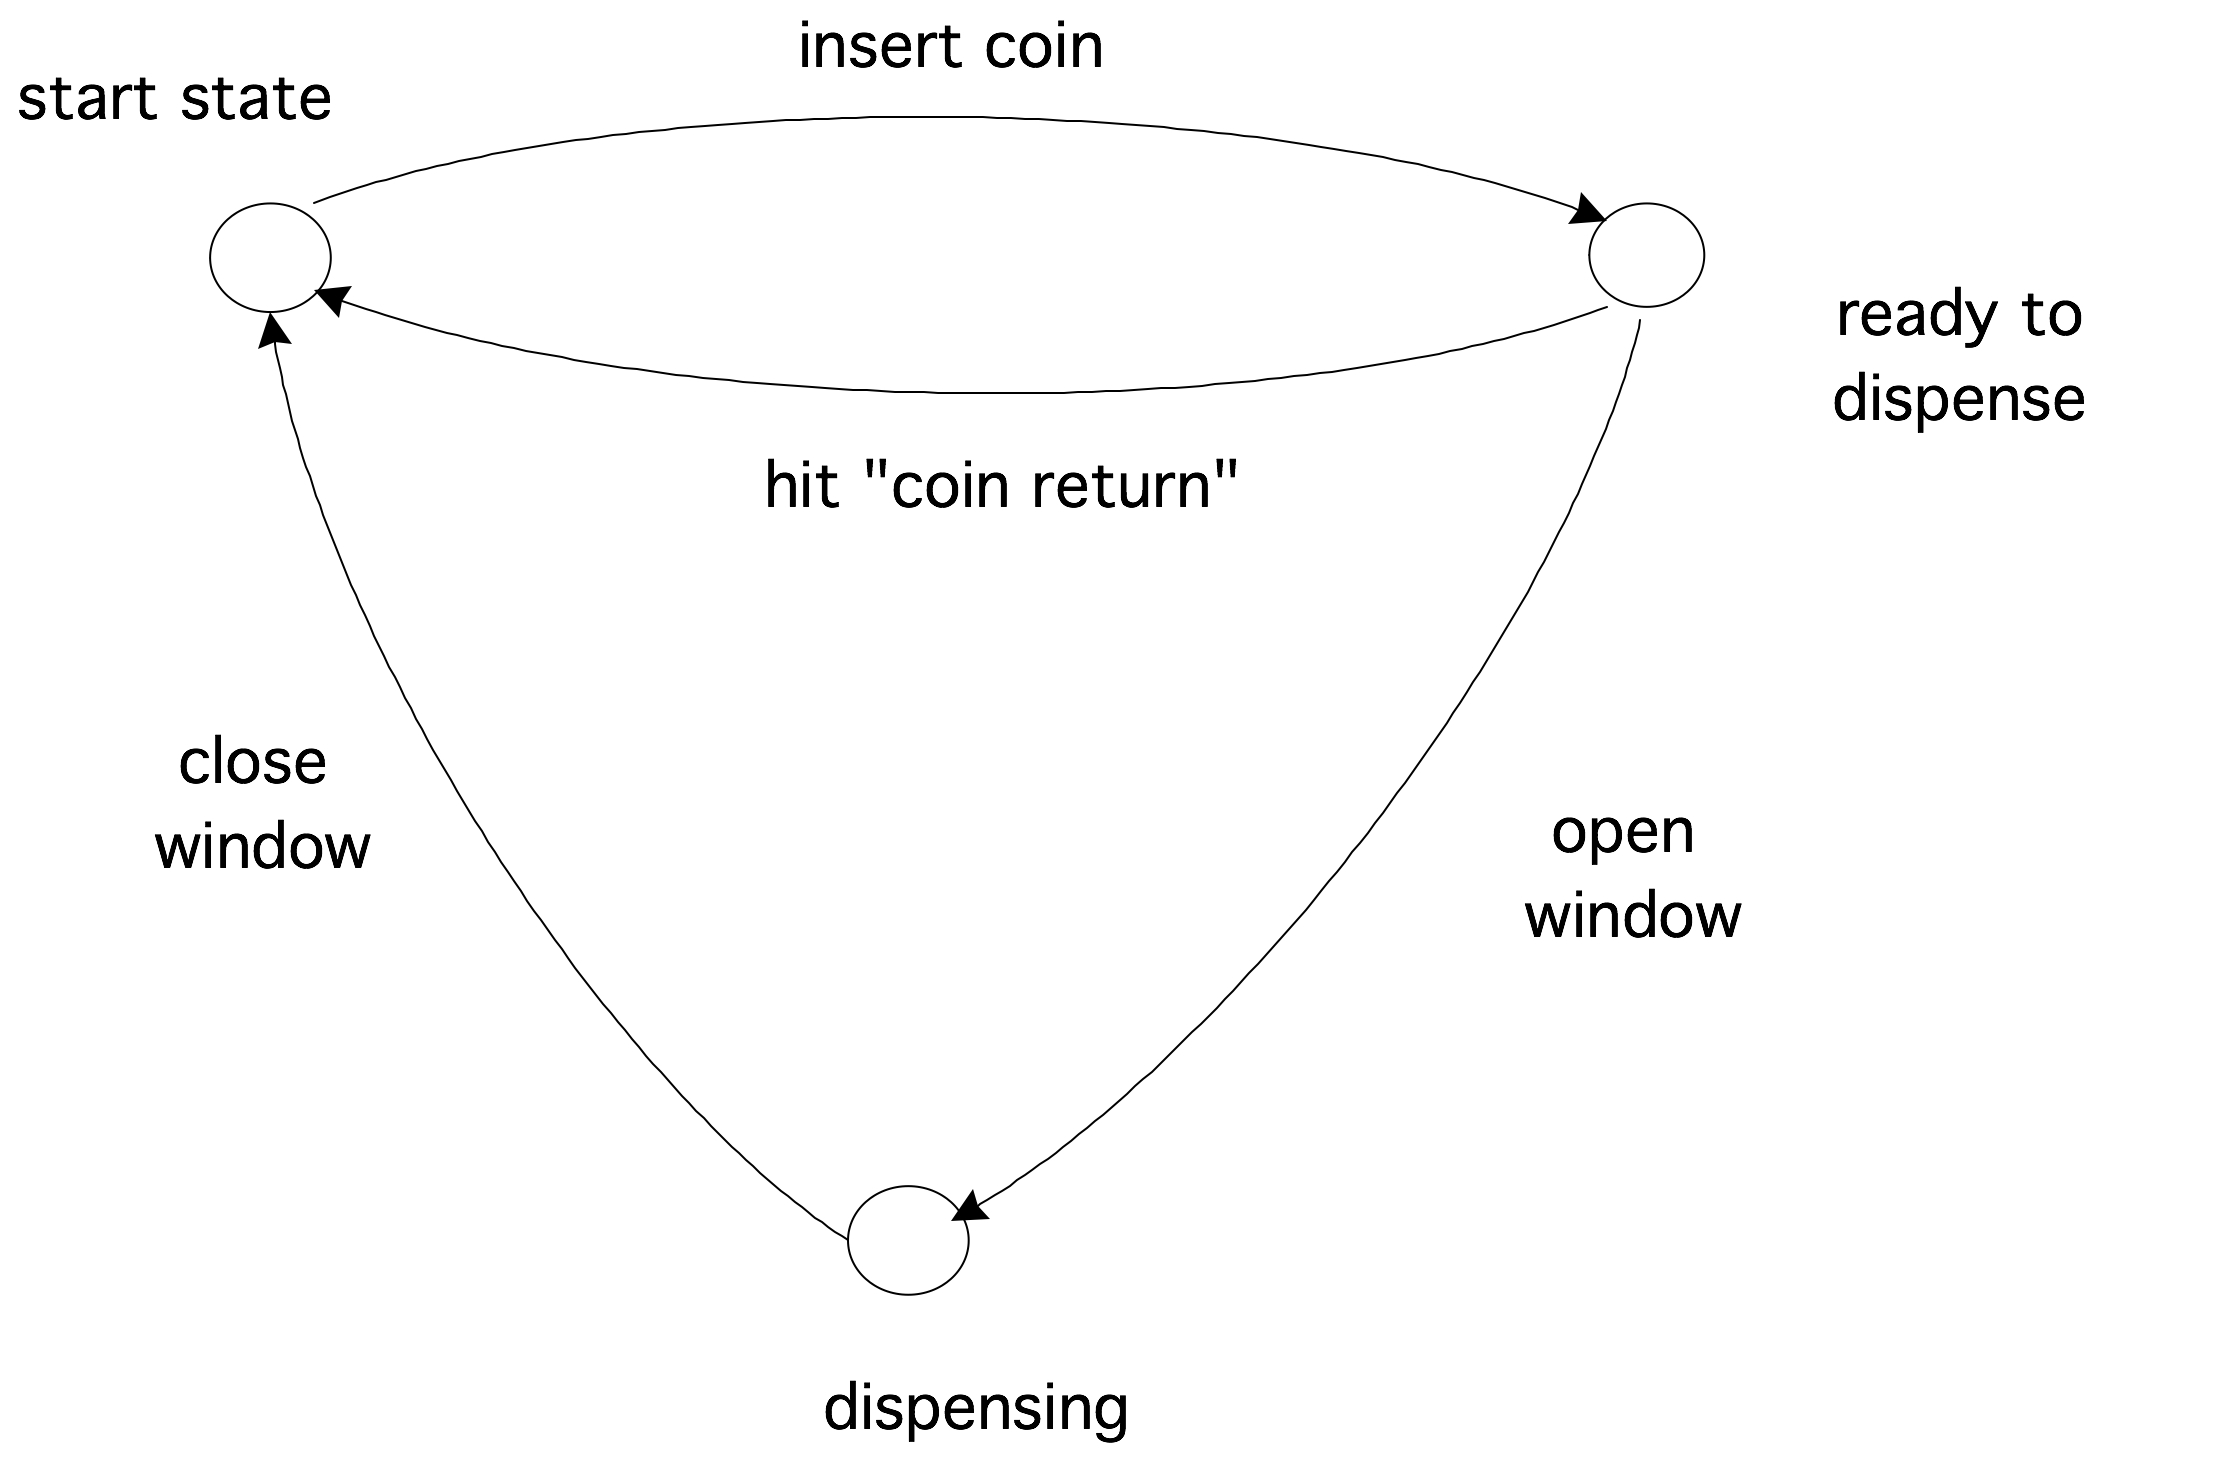
\includegraphics[scale=.15]{fsa}
  \caption{A simple real-life automaton.}
  \label{fig:automaton}
\end{figure}

\Level 0 {General discussion}

From the vending machine example, you saw an important characteristic of an automaton: 
it allows certain actions, but only in some circumstances, and in the end it has a 
state corresponding to `success', which is only reached if certain sequences of actions
are taken.

The formal description of this process is as follows: we call the
individual actions an `alphabet', and a sequence of actions a `word'
from based on that alphabet. The `success' result of a machine then
corresponds to a verdict that a certain word belong to the `language'
that is accepted by the automaton. Thus there is a correspondence
between automata theory and language theory.

\begin{exercise}
Consider the alpha $\{a,b\}$, that is, the alphabet with only the
letters $a,b$, and consider the language $\{a^mb^n\colon m,n>0\}$,
that is the words that consist of one or more $a$s followed by one or
more~$b$s. Draw the automaton that accepts this language.
\end{exercise}

What makes the \ac{FSA} the simplest type is that it has no
memory. Most vending machines do not complain if you put in more than
one quarter: they have no memory beyond `a~quarter has been
inserted'. A more complicated machine would count how many quarters
you inserted, and then allow you to open that many windows to
different candy bars. In the above formal way of describing, that
machine would accept the language $\{q^nw^n\colon n\geq 0\}$, that is,
the sequences where you deposit as many quarters (`$q$') as you open
windows~(`$w$'). This language is an example of a
so-called \indextermsub{context-free}{language}; the language of the
original vending machine is a \indextermsub{regular}{language}.

These two language types belong to the four level \indexterm{Chomsky
hierarchy} of languages. The famous \indexterm{Turing machine}, which
recognizes the \indextermsub{recursively enumerable}{language} type, is on the
top level of the hierarchy. The missing step has
the \indextermsub{context-sensitive}{language} type, which is
recognized by a \indextermsub{linear bounded}{automaton}.


\index{automaton|)}
\endinput

\begingroup\raggedright
\begin{tabular}{p{1.2in}p{1.2in}p{1.2in}p{1.2in}}
  \hfill state:&begin state&accepting&dispensing\\
  action:\\
  insert coin&go to accepting state&go to dispensing state\\
  take candy:&&&go back to begin state
\end{tabular}
\endgroup
